\documentclass[fleqn]{article}

\usepackage{polski}
\usepackage[utf8]{inputenc}
\usepackage[polish]{babel}
\usepackage{parskip}
\usepackage{icomma}
\usepackage[a4paper,includeheadfoot,margin=1.27cm]{geometry}
\usepackage{float}
\usepackage{graphicx}
\usepackage{amsmath}
\usepackage[hypcap=true]{subcaption}
\usepackage{xcolor}
\usepackage{transparent}
\usepackage{listings}
\usepackage[colorlinks=true, linkcolor=blue, pdfborder={0 0 0}]{hyperref}

\renewcommand\thesection{\arabic{section}.}
\renewcommand\thesubsection{\alph{subsection})}
\renewcommand\thesubsubsection{}
\newcommand\square[1]{
	\fcolorbox{black}{#1}{\rule{0pt}{6pt}\rule{6pt}{0pt}}
}

\brokenpenalty=1000
\clubpenalty=1000
\widowpenalty=1000

\title{TM -- Laboratorium 2. \\ \large Licznik 4-bitowy – zerowanie, zliczanie w górę – kod NKB}
\author{Krystian Chachuła \\ Dawid Gruszczyński \\ Marcin Skrzypkowski}

\begin{document}

\maketitle

\setcounter{page}{0}
\thispagestyle{empty}

\pagebreak

\setcounter{page}{1}

\section{Wstęp}

Na drugim laboratorium mieliśmy za zadanie zaprojektować i zrealizować licznik zliczający w górę w kodzie NKB z możliwością asynchronicznego zerowania jego zawartości.
Sterowanie licznikiem miało odbywać się za pomocą dwóch przycisków (CLK aktywne zboczem oraz CLR aktywne poziomem).
Dodatkowym wymogiem zadania była realizacja programowej eliminacji drgań styków oraz zerowania licznika za pomocą przerwania maskowalnego.

Zaprojektowany przed laboratorium układ zbudowaliśmy z następujących układów SML-3:

\begin{itemize}
	\item \textbf{10\_PS1} (moduł zasilacza)
	\item \textbf{100\_LED8} (zestaw 8 diod)
	\item \textbf{120\_IN8} (zestaw 8 monostabilnych wyłączników)
	\item \textbf{202\_NAND} (zestaw bramek \textit{NAND})
	\item \textbf{380\_NOTx6} (moduł sześciu bramek negujących)
	\item procesor Z80 zrealizowany w układzie FPGA
\end{itemize}

\section{Implementacja licznika}

Projektowanie licznika rozpoczęliśmy od stworzenia grafu stanów, który uwzględniał aktywną eliminację drgań styków przycisku zliczającego.
Graf składa się z 4 stanów. W stanie początkowym układ oczekuje na wciśnięcie przycisku, w stanie drugim eliminowane są drgania związanie z wciśnięciem przycisku, w stanie trzecim układ oczekuje na puszczenie przycisku, w stanie 4 eliminowane są drgania związanie z puszczeniem przycisku.
%TODO ogarnąć grafuu

\begin{figure}[H]
	\centering
	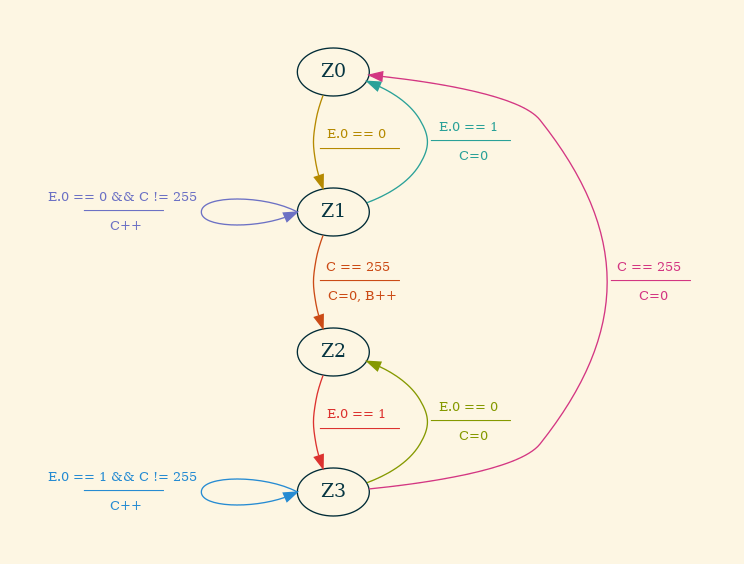
\includegraphics[width=0.72\textwidth]{img/graph.png}
	\caption{Graf automatu stanów}
	\label{fig:graph}
\end{figure}

Następnie na podstawie grafu powstał kod napisany w języku Assembly.

%TODO  trzeba będzie zrobić opis
\noindent\begin{minipage}{.45\textwidth}
	\lstinputlisting[lastline=50]{src/main.lst}
\end{minipage}\hfill
\noindent\begin{minipage}{.45\textwidth}
	\lstinputlisting[firstline=51]{src/main.lst}
\end{minipage}\hfill

Schemat połączeń wygląda następująco:
%TODO wstawić Schemat


Przycisk odpowiedzialny za zliczanie został podłączony do wejścia D0 rejestru wejściowego C, natomiast przycisk odpowiedzialny za asynchroniczne zerowanie do wejścia $\overline{INT}$ procesora.
Wyświetlanie zawartości licznika odbywa się za pomocą rejestru wyjściowego A, którego wyjścia podłączone są do modułu diod SML-3 $\textit{100\_LED8}$. Rejestry A i C podłączone są do procesora w taki sposób by reagowały tylko na operacje zapisu do przestrzeni wejścia/wyjścia (rejestr B) lub odczytu (rejestr C), a więc wyświetlanie zawartości oraz odczyt stanu przycisku zliczającego.


\section{Problemy}
W trakcie pracy nad licznikiem natrafiliśmy na problem związany z organizacją kodu w przestrzeni pamięciowej procesora Z80 (dobrze to sformułowałem? xD), napisany przez nas kod wykorzystujący (polecenie/dyrektywę czy jak to się zwie) ORG /adres/ w celu umieszczenia bloku kodu w oddzielnym miejscu w pamięci nie było uwzględniane w pliku kompilacyjnym (proszę poprawcie wszystko co napisałem źle, kompletnie się na tym nie znam xD), przez co cały sklejony kod lądował pod adresem 1800h. Rozwiązaliśmy ten problem za pomocą zapełniania komórek pamięci zerami (kodami instrukcji NOP), pozwoliło nam to na odpowiednią organizację kodu w pamięci, ponieważ niewykorzystywane przez nas komórki pamięci np. pomiędzy adresem 1802h a 1838h po zapełnieniu zerami za pomocą instrukcji DS cośtam pozwoliły na zapisanie kodu obsługi przerwania w odpowiednim miejscu (pod adresem 1838h).
\end{document}
